% Created by tikzDevice version 0.12 on 2019-05-23 20:15:37
% !TEX encoding = UTF-8 Unicode
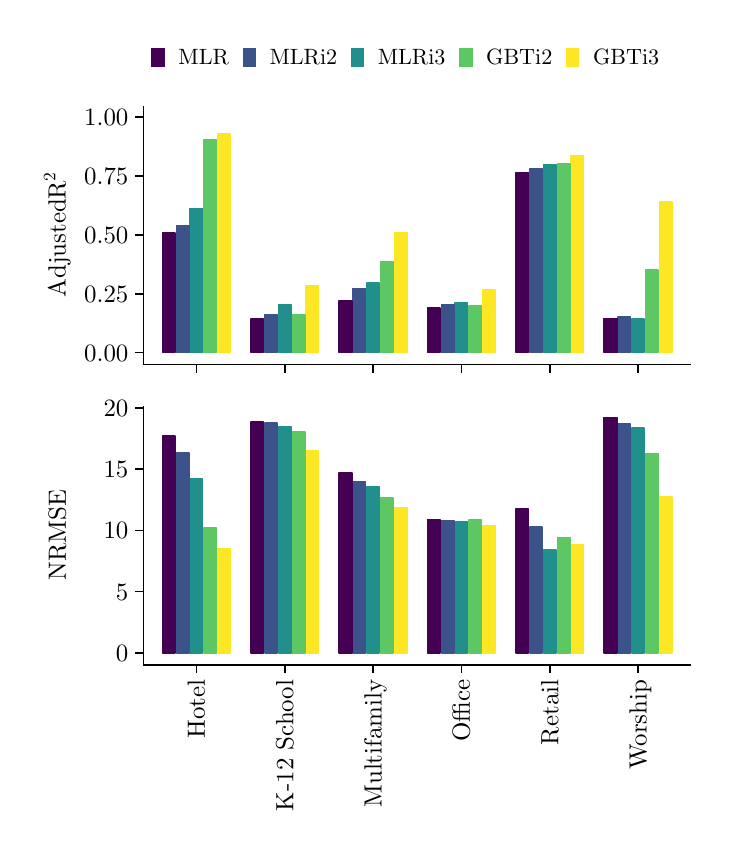
\begin{tikzpicture}[x=1pt,y=1pt]
\definecolor{fillColor}{RGB}{255,255,255}
\path[use as bounding box,fill=fillColor,fill opacity=0.00] (0,0) rectangle (245.72,289.08);
\begin{scope}
\path[clip] (  0.00,158.41) rectangle (245.72,289.08);
\definecolor{drawColor}{RGB}{255,255,255}
\definecolor{fillColor}{RGB}{255,255,255}

\path[draw=drawColor,line width= 0.6pt,line join=round,line cap=round,fill=fillColor] (  0.00,158.41) rectangle (245.72,289.08);
\end{scope}
\begin{scope}
\path[clip] (  0.00,  0.00) rectangle (245.72,158.41);
\definecolor{drawColor}{RGB}{255,255,255}
\definecolor{fillColor}{RGB}{255,255,255}

\path[draw=drawColor,line width= 0.6pt,line join=round,line cap=round,fill=fillColor] (  0.00,  0.00) rectangle (245.72,158.41);
\end{scope}
\begin{scope}
\path[clip] ( 41.81,167.41) rectangle (239.72,260.94);
\definecolor{fillColor}{RGB}{255,255,255}

\path[fill=fillColor] ( 41.81,167.41) rectangle (239.72,260.94);
\definecolor{drawColor}{RGB}{253,231,37}
\definecolor{fillColor}{RGB}{253,231,37}

\path[draw=drawColor,line width= 0.6pt,line join=round,fill=fillColor] ( 68.69,171.66) rectangle ( 73.16,250.73);
\definecolor{drawColor}{RGB}{93,200,99}
\definecolor{fillColor}{RGB}{93,200,99}

\path[draw=drawColor,line width= 0.6pt,line join=round,fill=fillColor] ( 63.71,171.66) rectangle ( 68.18,248.44);
\definecolor{drawColor}{RGB}{33,144,140}
\definecolor{fillColor}{RGB}{33,144,140}

\path[draw=drawColor,line width= 0.6pt,line join=round,fill=fillColor] ( 58.73,171.66) rectangle ( 63.20,223.78);
\definecolor{drawColor}{RGB}{59,82,139}
\definecolor{fillColor}{RGB}{59,82,139}

\path[draw=drawColor,line width= 0.6pt,line join=round,fill=fillColor] ( 53.75,171.66) rectangle ( 58.22,217.32);
\definecolor{drawColor}{RGB}{68,1,84}
\definecolor{fillColor}{RGB}{68,1,84}

\path[draw=drawColor,line width= 0.6pt,line join=round,fill=fillColor] ( 48.77,171.66) rectangle ( 53.24,214.77);
\definecolor{drawColor}{RGB}{253,231,37}
\definecolor{fillColor}{RGB}{253,231,37}

\path[draw=drawColor,line width= 0.6pt,line join=round,fill=fillColor] (100.61,171.66) rectangle (105.08,195.81);
\definecolor{drawColor}{RGB}{93,200,99}
\definecolor{fillColor}{RGB}{93,200,99}

\path[draw=drawColor,line width= 0.6pt,line join=round,fill=fillColor] ( 95.63,171.66) rectangle (100.10,185.35);
\definecolor{drawColor}{RGB}{33,144,140}
\definecolor{fillColor}{RGB}{33,144,140}

\path[draw=drawColor,line width= 0.6pt,line join=round,fill=fillColor] ( 90.65,171.66) rectangle ( 95.12,189.09);
\definecolor{drawColor}{RGB}{59,82,139}
\definecolor{fillColor}{RGB}{59,82,139}

\path[draw=drawColor,line width= 0.6pt,line join=round,fill=fillColor] ( 85.67,171.66) rectangle ( 90.14,185.44);
\definecolor{drawColor}{RGB}{68,1,84}
\definecolor{fillColor}{RGB}{68,1,84}

\path[draw=drawColor,line width= 0.6pt,line join=round,fill=fillColor] ( 80.69,171.66) rectangle ( 85.16,183.91);
\definecolor{drawColor}{RGB}{253,231,37}
\definecolor{fillColor}{RGB}{253,231,37}

\path[draw=drawColor,line width= 0.6pt,line join=round,fill=fillColor] (132.53,171.66) rectangle (137.00,215.11);
\definecolor{drawColor}{RGB}{93,200,99}
\definecolor{fillColor}{RGB}{93,200,99}

\path[draw=drawColor,line width= 0.6pt,line join=round,fill=fillColor] (127.55,171.66) rectangle (132.02,204.57);
\definecolor{drawColor}{RGB}{33,144,140}
\definecolor{fillColor}{RGB}{33,144,140}

\path[draw=drawColor,line width= 0.6pt,line join=round,fill=fillColor] (122.57,171.66) rectangle (127.04,196.92);
\definecolor{drawColor}{RGB}{59,82,139}
\definecolor{fillColor}{RGB}{59,82,139}

\path[draw=drawColor,line width= 0.6pt,line join=round,fill=fillColor] (117.59,171.66) rectangle (122.06,194.79);
\definecolor{drawColor}{RGB}{68,1,84}
\definecolor{fillColor}{RGB}{68,1,84}

\path[draw=drawColor,line width= 0.6pt,line join=round,fill=fillColor] (112.61,171.66) rectangle (117.08,190.37);
\definecolor{drawColor}{RGB}{253,231,37}
\definecolor{fillColor}{RGB}{253,231,37}

\path[draw=drawColor,line width= 0.6pt,line join=round,fill=fillColor] (164.45,171.66) rectangle (168.92,194.36);
\definecolor{drawColor}{RGB}{93,200,99}
\definecolor{fillColor}{RGB}{93,200,99}

\path[draw=drawColor,line width= 0.6pt,line join=round,fill=fillColor] (159.47,171.66) rectangle (163.94,188.58);
\definecolor{drawColor}{RGB}{33,144,140}
\definecolor{fillColor}{RGB}{33,144,140}

\path[draw=drawColor,line width= 0.6pt,line join=round,fill=fillColor] (154.49,171.66) rectangle (158.96,189.69);
\definecolor{drawColor}{RGB}{59,82,139}
\definecolor{fillColor}{RGB}{59,82,139}

\path[draw=drawColor,line width= 0.6pt,line join=round,fill=fillColor] (149.51,171.66) rectangle (153.98,189.01);
\definecolor{drawColor}{RGB}{68,1,84}
\definecolor{fillColor}{RGB}{68,1,84}

\path[draw=drawColor,line width= 0.6pt,line join=round,fill=fillColor] (144.53,171.66) rectangle (149.00,187.90);
\definecolor{drawColor}{RGB}{253,231,37}
\definecolor{fillColor}{RGB}{253,231,37}

\path[draw=drawColor,line width= 0.6pt,line join=round,fill=fillColor] (196.37,171.66) rectangle (200.84,242.83);
\definecolor{drawColor}{RGB}{93,200,99}
\definecolor{fillColor}{RGB}{93,200,99}

\path[draw=drawColor,line width= 0.6pt,line join=round,fill=fillColor] (191.39,171.66) rectangle (195.86,239.77);
\definecolor{drawColor}{RGB}{33,144,140}
\definecolor{fillColor}{RGB}{33,144,140}

\path[draw=drawColor,line width= 0.6pt,line join=round,fill=fillColor] (186.41,171.66) rectangle (190.88,239.60);
\definecolor{drawColor}{RGB}{59,82,139}
\definecolor{fillColor}{RGB}{59,82,139}

\path[draw=drawColor,line width= 0.6pt,line join=round,fill=fillColor] (181.43,171.66) rectangle (185.90,238.24);
\definecolor{drawColor}{RGB}{68,1,84}
\definecolor{fillColor}{RGB}{68,1,84}

\path[draw=drawColor,line width= 0.6pt,line join=round,fill=fillColor] (176.45,171.66) rectangle (180.92,236.79);
\definecolor{drawColor}{RGB}{253,231,37}
\definecolor{fillColor}{RGB}{253,231,37}

\path[draw=drawColor,line width= 0.6pt,line join=round,fill=fillColor] (228.29,171.66) rectangle (232.76,225.99);
\definecolor{drawColor}{RGB}{93,200,99}
\definecolor{fillColor}{RGB}{93,200,99}

\path[draw=drawColor,line width= 0.6pt,line join=round,fill=fillColor] (223.31,171.66) rectangle (227.78,201.51);
\definecolor{drawColor}{RGB}{33,144,140}
\definecolor{fillColor}{RGB}{33,144,140}

\path[draw=drawColor,line width= 0.6pt,line join=round,fill=fillColor] (218.33,171.66) rectangle (222.80,183.74);
\definecolor{drawColor}{RGB}{59,82,139}
\definecolor{fillColor}{RGB}{59,82,139}

\path[draw=drawColor,line width= 0.6pt,line join=round,fill=fillColor] (213.35,171.66) rectangle (217.82,184.50);
\definecolor{drawColor}{RGB}{68,1,84}
\definecolor{fillColor}{RGB}{68,1,84}

\path[draw=drawColor,line width= 0.6pt,line join=round,fill=fillColor] (208.37,171.66) rectangle (212.84,183.99);
\end{scope}
\begin{scope}
\path[clip] ( 41.81, 58.89) rectangle (239.72,152.41);
\definecolor{fillColor}{RGB}{255,255,255}

\path[fill=fillColor] ( 41.81, 58.89) rectangle (239.72,152.41);
\definecolor{drawColor}{RGB}{253,231,37}
\definecolor{fillColor}{RGB}{253,231,37}

\path[draw=drawColor,line width= 0.6pt,line join=round,fill=fillColor] ( 68.69, 63.14) rectangle ( 73.16,100.86);
\definecolor{drawColor}{RGB}{93,200,99}
\definecolor{fillColor}{RGB}{93,200,99}

\path[draw=drawColor,line width= 0.6pt,line join=round,fill=fillColor] ( 63.71, 63.14) rectangle ( 68.18,108.21);
\definecolor{drawColor}{RGB}{33,144,140}
\definecolor{fillColor}{RGB}{33,144,140}

\path[draw=drawColor,line width= 0.6pt,line join=round,fill=fillColor] ( 58.73, 63.14) rectangle ( 63.20,126.03);
\definecolor{drawColor}{RGB}{59,82,139}
\definecolor{fillColor}{RGB}{59,82,139}

\path[draw=drawColor,line width= 0.6pt,line join=round,fill=fillColor] ( 53.75, 63.14) rectangle ( 58.22,135.49);
\definecolor{drawColor}{RGB}{68,1,84}
\definecolor{fillColor}{RGB}{68,1,84}

\path[draw=drawColor,line width= 0.6pt,line join=round,fill=fillColor] ( 48.77, 63.14) rectangle ( 53.24,141.58);
\definecolor{drawColor}{RGB}{253,231,37}
\definecolor{fillColor}{RGB}{253,231,37}

\path[draw=drawColor,line width= 0.6pt,line join=round,fill=fillColor] (100.61, 63.14) rectangle (105.08,136.03);
\definecolor{drawColor}{RGB}{93,200,99}
\definecolor{fillColor}{RGB}{93,200,99}

\path[draw=drawColor,line width= 0.6pt,line join=round,fill=fillColor] ( 95.63, 63.14) rectangle (100.10,142.87);
\definecolor{drawColor}{RGB}{33,144,140}
\definecolor{fillColor}{RGB}{33,144,140}

\path[draw=drawColor,line width= 0.6pt,line join=round,fill=fillColor] ( 90.65, 63.14) rectangle ( 95.12,144.97);
\definecolor{drawColor}{RGB}{59,82,139}
\definecolor{fillColor}{RGB}{59,82,139}

\path[draw=drawColor,line width= 0.6pt,line join=round,fill=fillColor] ( 85.67, 63.14) rectangle ( 90.14,146.23);
\definecolor{drawColor}{RGB}{68,1,84}
\definecolor{fillColor}{RGB}{68,1,84}

\path[draw=drawColor,line width= 0.6pt,line join=round,fill=fillColor] ( 80.69, 63.14) rectangle ( 85.16,146.63);
\definecolor{drawColor}{RGB}{253,231,37}
\definecolor{fillColor}{RGB}{253,231,37}

\path[draw=drawColor,line width= 0.6pt,line join=round,fill=fillColor] (132.53, 63.14) rectangle (137.00,115.71);
\definecolor{drawColor}{RGB}{93,200,99}
\definecolor{fillColor}{RGB}{93,200,99}

\path[draw=drawColor,line width= 0.6pt,line join=round,fill=fillColor] (127.55, 63.14) rectangle (132.02,119.19);
\definecolor{drawColor}{RGB}{33,144,140}
\definecolor{fillColor}{RGB}{33,144,140}

\path[draw=drawColor,line width= 0.6pt,line join=round,fill=fillColor] (122.57, 63.14) rectangle (127.04,123.30);
\definecolor{drawColor}{RGB}{59,82,139}
\definecolor{fillColor}{RGB}{59,82,139}

\path[draw=drawColor,line width= 0.6pt,line join=round,fill=fillColor] (117.59, 63.14) rectangle (122.06,125.03);
\definecolor{drawColor}{RGB}{68,1,84}
\definecolor{fillColor}{RGB}{68,1,84}

\path[draw=drawColor,line width= 0.6pt,line join=round,fill=fillColor] (112.61, 63.14) rectangle (117.08,128.04);
\definecolor{drawColor}{RGB}{253,231,37}
\definecolor{fillColor}{RGB}{253,231,37}

\path[draw=drawColor,line width= 0.6pt,line join=round,fill=fillColor] (164.45, 63.14) rectangle (168.92,109.17);
\definecolor{drawColor}{RGB}{93,200,99}
\definecolor{fillColor}{RGB}{93,200,99}

\path[draw=drawColor,line width= 0.6pt,line join=round,fill=fillColor] (159.47, 63.14) rectangle (163.94,111.18);
\definecolor{drawColor}{RGB}{33,144,140}
\definecolor{fillColor}{RGB}{33,144,140}

\path[draw=drawColor,line width= 0.6pt,line join=round,fill=fillColor] (154.49, 63.14) rectangle (158.96,110.60);
\definecolor{drawColor}{RGB}{59,82,139}
\definecolor{fillColor}{RGB}{59,82,139}

\path[draw=drawColor,line width= 0.6pt,line join=round,fill=fillColor] (149.51, 63.14) rectangle (153.98,110.99);
\definecolor{drawColor}{RGB}{68,1,84}
\definecolor{fillColor}{RGB}{68,1,84}

\path[draw=drawColor,line width= 0.6pt,line join=round,fill=fillColor] (144.53, 63.14) rectangle (149.00,111.41);
\definecolor{drawColor}{RGB}{253,231,37}
\definecolor{fillColor}{RGB}{253,231,37}

\path[draw=drawColor,line width= 0.6pt,line join=round,fill=fillColor] (196.37, 63.14) rectangle (200.84,102.11);
\definecolor{drawColor}{RGB}{93,200,99}
\definecolor{fillColor}{RGB}{93,200,99}

\path[draw=drawColor,line width= 0.6pt,line join=round,fill=fillColor] (191.39, 63.14) rectangle (195.86,104.87);
\definecolor{drawColor}{RGB}{33,144,140}
\definecolor{fillColor}{RGB}{33,144,140}

\path[draw=drawColor,line width= 0.6pt,line join=round,fill=fillColor] (186.41, 63.14) rectangle (190.88,100.40);
\definecolor{drawColor}{RGB}{59,82,139}
\definecolor{fillColor}{RGB}{59,82,139}

\path[draw=drawColor,line width= 0.6pt,line join=round,fill=fillColor] (181.43, 63.14) rectangle (185.90,108.55);
\definecolor{drawColor}{RGB}{68,1,84}
\definecolor{fillColor}{RGB}{68,1,84}

\path[draw=drawColor,line width= 0.6pt,line join=round,fill=fillColor] (176.45, 63.14) rectangle (180.92,115.11);
\definecolor{drawColor}{RGB}{253,231,37}
\definecolor{fillColor}{RGB}{253,231,37}

\path[draw=drawColor,line width= 0.6pt,line join=round,fill=fillColor] (228.29, 63.14) rectangle (232.76,119.53);
\definecolor{drawColor}{RGB}{93,200,99}
\definecolor{fillColor}{RGB}{93,200,99}

\path[draw=drawColor,line width= 0.6pt,line join=round,fill=fillColor] (223.31, 63.14) rectangle (227.78,135.15);
\definecolor{drawColor}{RGB}{33,144,140}
\definecolor{fillColor}{RGB}{33,144,140}

\path[draw=drawColor,line width= 0.6pt,line join=round,fill=fillColor] (218.33, 63.14) rectangle (222.80,144.44);
\definecolor{drawColor}{RGB}{59,82,139}
\definecolor{fillColor}{RGB}{59,82,139}

\path[draw=drawColor,line width= 0.6pt,line join=round,fill=fillColor] (213.35, 63.14) rectangle (217.82,145.93);
\definecolor{drawColor}{RGB}{68,1,84}
\definecolor{fillColor}{RGB}{68,1,84}

\path[draw=drawColor,line width= 0.6pt,line join=round,fill=fillColor] (208.37, 63.14) rectangle (212.84,148.16);
\end{scope}
\begin{scope}
\path[clip] (  0.00,  0.00) rectangle (245.72,289.08);
\definecolor{drawColor}{RGB}{0,0,0}

\path[draw=drawColor,line width= 0.6pt,line join=round] ( 41.81,167.41) --
	( 41.81,260.94);
\end{scope}
\begin{scope}
\path[clip] (  0.00,  0.00) rectangle (245.72,289.08);
\definecolor{drawColor}{RGB}{0,0,0}

\node[text=drawColor,anchor=base east,inner sep=0pt, outer sep=0pt, scale=  0.90] at ( 36.41,168.56) {0.00};

\node[text=drawColor,anchor=base east,inner sep=0pt, outer sep=0pt, scale=  0.90] at ( 36.41,189.82) {0.25};

\node[text=drawColor,anchor=base east,inner sep=0pt, outer sep=0pt, scale=  0.90] at ( 36.41,211.08) {0.50};

\node[text=drawColor,anchor=base east,inner sep=0pt, outer sep=0pt, scale=  0.90] at ( 36.41,232.33) {0.75};

\node[text=drawColor,anchor=base east,inner sep=0pt, outer sep=0pt, scale=  0.90] at ( 36.41,253.59) {1.00};
\end{scope}
\begin{scope}
\path[clip] (  0.00,  0.00) rectangle (245.72,289.08);
\definecolor{drawColor}{RGB}{0,0,0}

\path[draw=drawColor,line width= 0.6pt,line join=round] ( 38.81,171.66) --
	( 41.81,171.66);

\path[draw=drawColor,line width= 0.6pt,line join=round] ( 38.81,192.92) --
	( 41.81,192.92);

\path[draw=drawColor,line width= 0.6pt,line join=round] ( 38.81,214.18) --
	( 41.81,214.18);

\path[draw=drawColor,line width= 0.6pt,line join=round] ( 38.81,235.43) --
	( 41.81,235.43);

\path[draw=drawColor,line width= 0.6pt,line join=round] ( 38.81,256.69) --
	( 41.81,256.69);
\end{scope}
\begin{scope}
\path[clip] (  0.00,  0.00) rectangle (245.72,289.08);
\definecolor{drawColor}{RGB}{0,0,0}

\path[draw=drawColor,line width= 0.6pt,line join=round] ( 41.81, 58.89) --
	( 41.81,152.41);
\end{scope}
\begin{scope}
\path[clip] (  0.00,  0.00) rectangle (245.72,289.08);
\definecolor{drawColor}{RGB}{0,0,0}

\node[text=drawColor,anchor=base east,inner sep=0pt, outer sep=0pt, scale=  0.90] at ( 36.41, 60.04) {0};

\node[text=drawColor,anchor=base east,inner sep=0pt, outer sep=0pt, scale=  0.90] at ( 36.41, 82.18) {5};

\node[text=drawColor,anchor=base east,inner sep=0pt, outer sep=0pt, scale=  0.90] at ( 36.41,104.33) {10};

\node[text=drawColor,anchor=base east,inner sep=0pt, outer sep=0pt, scale=  0.90] at ( 36.41,126.47) {15};

\node[text=drawColor,anchor=base east,inner sep=0pt, outer sep=0pt, scale=  0.90] at ( 36.41,148.61) {20};
\end{scope}
\begin{scope}
\path[clip] (  0.00,  0.00) rectangle (245.72,289.08);
\definecolor{drawColor}{RGB}{0,0,0}

\path[draw=drawColor,line width= 0.6pt,line join=round] ( 38.81, 63.14) --
	( 41.81, 63.14);

\path[draw=drawColor,line width= 0.6pt,line join=round] ( 38.81, 85.28) --
	( 41.81, 85.28);

\path[draw=drawColor,line width= 0.6pt,line join=round] ( 38.81,107.43) --
	( 41.81,107.43);

\path[draw=drawColor,line width= 0.6pt,line join=round] ( 38.81,129.57) --
	( 41.81,129.57);

\path[draw=drawColor,line width= 0.6pt,line join=round] ( 38.81,151.71) --
	( 41.81,151.71);
\end{scope}
\begin{scope}
\path[clip] (  0.00,  0.00) rectangle (245.72,289.08);
\definecolor{drawColor}{RGB}{0,0,0}

\path[draw=drawColor,line width= 0.6pt,line join=round] ( 41.81,167.41) --
	(239.72,167.41);
\end{scope}
\begin{scope}
\path[clip] (  0.00,  0.00) rectangle (245.72,289.08);
\definecolor{drawColor}{RGB}{0,0,0}

\path[draw=drawColor,line width= 0.6pt,line join=round] ( 60.96,164.41) --
	( 60.96,167.41);

\path[draw=drawColor,line width= 0.6pt,line join=round] ( 92.88,164.41) --
	( 92.88,167.41);

\path[draw=drawColor,line width= 0.6pt,line join=round] (124.80,164.41) --
	(124.80,167.41);

\path[draw=drawColor,line width= 0.6pt,line join=round] (156.72,164.41) --
	(156.72,167.41);

\path[draw=drawColor,line width= 0.6pt,line join=round] (188.65,164.41) --
	(188.65,167.41);

\path[draw=drawColor,line width= 0.6pt,line join=round] (220.57,164.41) --
	(220.57,167.41);
\end{scope}
\begin{scope}
\path[clip] (  0.00,  0.00) rectangle (245.72,289.08);
\definecolor{drawColor}{RGB}{0,0,0}

\path[draw=drawColor,line width= 0.6pt,line join=round] ( 41.81, 58.89) --
	(239.72, 58.89);
\end{scope}
\begin{scope}
\path[clip] (  0.00,  0.00) rectangle (245.72,289.08);
\definecolor{drawColor}{RGB}{0,0,0}

\path[draw=drawColor,line width= 0.6pt,line join=round] ( 60.96, 55.89) --
	( 60.96, 58.89);

\path[draw=drawColor,line width= 0.6pt,line join=round] ( 92.88, 55.89) --
	( 92.88, 58.89);

\path[draw=drawColor,line width= 0.6pt,line join=round] (124.80, 55.89) --
	(124.80, 58.89);

\path[draw=drawColor,line width= 0.6pt,line join=round] (156.72, 55.89) --
	(156.72, 58.89);

\path[draw=drawColor,line width= 0.6pt,line join=round] (188.65, 55.89) --
	(188.65, 58.89);

\path[draw=drawColor,line width= 0.6pt,line join=round] (220.57, 55.89) --
	(220.57, 58.89);
\end{scope}
\begin{scope}
\path[clip] (  0.00,  0.00) rectangle (245.72,289.08);
\definecolor{drawColor}{RGB}{0,0,0}

\node[text=drawColor,rotate= 90.00,anchor=base east,inner sep=0pt, outer sep=0pt, scale=  0.90] at ( 64.06, 53.49) {Hotel};

\node[text=drawColor,rotate= 90.00,anchor=base east,inner sep=0pt, outer sep=0pt, scale=  0.90] at ( 95.98, 53.49) {K-12 School};

\node[text=drawColor,rotate= 90.00,anchor=base east,inner sep=0pt, outer sep=0pt, scale=  0.90] at (127.90, 53.49) {Multifamily};

\node[text=drawColor,rotate= 90.00,anchor=base east,inner sep=0pt, outer sep=0pt, scale=  0.90] at (159.82, 53.49) {Office};

\node[text=drawColor,rotate= 90.00,anchor=base east,inner sep=0pt, outer sep=0pt, scale=  0.90] at (191.74, 53.49) {Retail};

\node[text=drawColor,rotate= 90.00,anchor=base east,inner sep=0pt, outer sep=0pt, scale=  0.90] at (223.66, 53.49) {Worship};
\end{scope}
\begin{scope}
\path[clip] (  0.00,  0.00) rectangle (245.72,289.08);
\definecolor{drawColor}{RGB}{0,0,0}

\node[text=drawColor,rotate= 90.00,anchor=base west,inner sep=0pt, outer sep=0pt, scale=  0.90] at ( 13.72,191.64) {Adjusted };

\node[text=drawColor,rotate= 90.00,anchor=base west,inner sep=0pt, outer sep=0pt, scale=  0.90] at ( 13.72,226.93) {R};

\node[text=drawColor,rotate= 90.00,anchor=base west,inner sep=0pt, outer sep=0pt, scale=  0.63] at ( 10.04,233.56) {2};
\end{scope}
\begin{scope}
\path[clip] (  0.00,  0.00) rectangle (245.72,289.08);
\definecolor{drawColor}{RGB}{0,0,0}

\node[text=drawColor,rotate= 90.00,anchor=base,inner sep=0pt, outer sep=0pt, scale=  0.90] at ( 13.83,105.65) {NRMSE};
\end{scope}
\begin{scope}
\path[clip] (  0.00,  0.00) rectangle (245.72,289.08);
\definecolor{fillColor}{RGB}{255,255,255}

\path[fill=fillColor] ( 40.81,272.94) rectangle (229.24,283.08);
\end{scope}
\begin{scope}
\path[clip] (  0.00,  0.00) rectangle (245.72,289.08);
\definecolor{drawColor}{RGB}{68,1,84}
\definecolor{fillColor}{RGB}{68,1,84}

\path[draw=drawColor,line width= 0.6pt,line cap=round,fill=fillColor] ( 45.02,275.34) rectangle ( 49.29,281.37);
\end{scope}
\begin{scope}
\path[clip] (  0.00,  0.00) rectangle (245.72,289.08);
\definecolor{drawColor}{RGB}{59,82,139}
\definecolor{fillColor}{RGB}{59,82,139}

\path[draw=drawColor,line width= 0.6pt,line cap=round,fill=fillColor] ( 77.93,275.34) rectangle ( 82.20,281.37);
\end{scope}
\begin{scope}
\path[clip] (  0.00,  0.00) rectangle (245.72,289.08);
\definecolor{drawColor}{RGB}{33,144,140}
\definecolor{fillColor}{RGB}{33,144,140}

\path[draw=drawColor,line width= 0.6pt,line cap=round,fill=fillColor] (117.06,275.34) rectangle (121.33,281.37);
\end{scope}
\begin{scope}
\path[clip] (  0.00,  0.00) rectangle (245.72,289.08);
\definecolor{drawColor}{RGB}{93,200,99}
\definecolor{fillColor}{RGB}{93,200,99}

\path[draw=drawColor,line width= 0.6pt,line cap=round,fill=fillColor] (156.19,275.34) rectangle (160.46,281.37);
\end{scope}
\begin{scope}
\path[clip] (  0.00,  0.00) rectangle (245.72,289.08);
\definecolor{drawColor}{RGB}{253,231,37}
\definecolor{fillColor}{RGB}{253,231,37}

\path[draw=drawColor,line width= 0.6pt,line cap=round,fill=fillColor] (194.82,275.34) rectangle (199.09,281.37);
\end{scope}
\begin{scope}
\path[clip] (  0.00,  0.00) rectangle (245.72,289.08);
\definecolor{drawColor}{RGB}{0,0,0}

\node[text=drawColor,anchor=base west,inner sep=0pt, outer sep=0pt, scale=  0.80] at ( 54.50,275.60) {MLR};
\end{scope}
\begin{scope}
\path[clip] (  0.00,  0.00) rectangle (245.72,289.08);
\definecolor{drawColor}{RGB}{0,0,0}

\node[text=drawColor,anchor=base west,inner sep=0pt, outer sep=0pt, scale=  0.80] at ( 87.41,275.60) {MLRi2};
\end{scope}
\begin{scope}
\path[clip] (  0.00,  0.00) rectangle (245.72,289.08);
\definecolor{drawColor}{RGB}{0,0,0}

\node[text=drawColor,anchor=base west,inner sep=0pt, outer sep=0pt, scale=  0.80] at (126.54,275.60) {MLRi3};
\end{scope}
\begin{scope}
\path[clip] (  0.00,  0.00) rectangle (245.72,289.08);
\definecolor{drawColor}{RGB}{0,0,0}

\node[text=drawColor,anchor=base west,inner sep=0pt, outer sep=0pt, scale=  0.80] at (165.67,275.60) {GBTi2};
\end{scope}
\begin{scope}
\path[clip] (  0.00,  0.00) rectangle (245.72,289.08);
\definecolor{drawColor}{RGB}{0,0,0}

\node[text=drawColor,anchor=base west,inner sep=0pt, outer sep=0pt, scale=  0.80] at (204.30,275.60) {GBTi3};
\end{scope}
\end{tikzpicture}
